% *********************************************************************
%    2016年 学士論文
% *********************************************************************
\documentclass[12pt,a4paper,titlepage]{jreport}

% 基本的なセット
\usepackage{graphicx,moreverb,amsmath,amsthm,amssymb}

% カスタム
\usepackage{comment,url}

% ソースコード掲載用
%\usepackage{listings,jlisting,ascmac,verbatim}

%\lstset{%
%  language={HTML},
%  % basicstyle={\footnotesize}
%  basicstyle={\small},%
%  identifierstyle={\small},%
%  commentstyle={\small\itshape},%
%  keywordstyle={\small\bfseries},%
%  ndkeywordstyle={\small},%
%  stringstyle={\small\ttfamily},
%  frame={tb},
%  % frame=trBL,
%  breaklines=true,
%  columns=[l]{fullflexible},%
%  numbers=left,%
%  xrightmargin=0zw,%
%  xleftmargin=3zw,%
%  numberstyle={\scriptsize},%
%  stepnumber=1,
%  numbersep=1zw,%
%  lineskip=-0.5ex%
%}

\setlength{\topmargin}{5pt}
\setlength{\oddsidemargin}{15pt}
\setlength{\evensidemargin}{15pt}
\setlength{\marginparwidth}{10pt}
\setlength{\textwidth}{30em}
\addtolength{\textwidth}{50pt}
\addtolength{\textheight}{50pt}

%------  ヘッダの飾り ------
\makeatletter
  \def\ps@testheadings{\let\@mkboth\markboth
  \def\@oddfoot{\hfil \rm\thepage \hfil}\def\@evenfoot{}
  \def\@oddhead{
   \underline{\hbox to 140mm{\hfil\rightmark}}}%\textwidth{\hfil\rightmark}}}
  \def\chaptermark##1{\markright {\uppercase{\ifnum \c@secnumdepth
  >\m@ne
  \@chapapp \ \fi ##1}}}}
\makeatother

\pagestyle{bothstyle}
\renewcommand{\bibname}{参考文献}
%--------------------------
\begin{document}
\pagenumbering{roman}
\baselineskip 22pt
%--------- 表紙 -----------------
\title{
\flushleft{\vspace{-3cm}\small{平成28年度~~卒業研究}}\\\vspace{3.5cm}
\center{{\huge \bf 機能語に注目した\\音声合成朗読システムのための\\感情推定手法の提案}}\vfill}
\author{
\rightline{東京理科大学~~理工学部~~経営工学科}\\
\rightline{西山研究室~~7413069~~恒川~~泰輝}\\
\rightline{}\\
\rightline{指導教員~~~西山~~裕之・金盛~~克俊}}
\date{}
\maketitle

%--------------------------------------------------
%     概要
%--------------------------------------------------
\chapter*{学士論文概要}
\addcontentsline{toc}{chapter}{学士論文概要}

%TODO 削減

%社会的背景
近年,従来の書籍の他に電子書籍など様々な書籍の楽しみ方が広がっている.
その中で,書籍の朗読は専門のナレーターによる朗読音声を収録したオーディオブックが知られている.
オーディオブックはアメリカを中心に市場規模が拡大している.
もともと車社会のアメリカなどの国では早期から市場が確立していたが,近年インターネットを介して気軽にダウンロードして楽しめる環境が整ったことなどによりアメリカとカナダの市場規模が2015年には前年比で約21\%拡大している\cite{wsj}.
日本においても定額配信サービスが開始されており,今後さらに普及する可能性がある.

しかし,このようなオーディオブックは書籍から音声化する際には手間やコストが電子書籍にくらべて10倍ほどかかっており2〜3ヶ月ほどかかると言われている.\cite{ueda}

%技術的・研究的背景・問題
そこで,電子書籍から人間の音声を人工的に作り出す音声合成技術を用いて機械で自動的に朗読するシステムの研究が行われている.
近年の音声合成技術を用いれば喜怒哀楽といった感情を指定することで感情豊かな音声を合成できる.
しかし,これらのパラメタは文もしくは単語ごとに人手で設定する必要がある.
短い文章など限られた場合は容易であるが,小説といった膨大な文章に対して都度人手でパラメタ調整を行うのは手間がかかる.

%目的
そこで本研究では未知の文に対しその文を読み上げるときの感情として最適なものを推測することを目的とする.
これにより自然な朗読システムが可能が実現可能になり,人手での手間やコストをかけずにオーディオブックを作成できるようになることが期待される.

%目的を達成するための手法
本研究では,文にどのような単語が含まれているかという出現情報をもとに機械学習技術を用いて感情を推定する.
名詞,動詞,形容,形容動詞は内容語とよばれるが物語に依存する可能性が高いため,内容を除いた機能語を用いることで内容に依存しない分類器を生成できる.
このため内容語を無視して機能語のみを用いて学習し感情の推定を行う.
セリフのみに限らずすべての文を対象に,出現情報から機能語に絞った感情推定を行っている研究は筆者の知る限り存在しない.

%実験手法の正しさの確認
本研究では,先行研究と同様にNormal,Happy,Sad,Angryの4つに感情をクラス分けする.
本手法の正しさを確認するための実験として,まず一つの文にそれぞれ4つの感情で音声を合成する.
そしてWebのアンケートシステムを用いて,被験者にこれらの音声を実際に聞いてもらい,その文を読み上げる際にどの感情が最も適しているか判定してもらう.
このように生成された学習データを用い交差検証を行うことで本手法の分類性能を評価する.

%-----------目次---------
\tableofcontents
\newpage
\listoffigures
\newpage
\listoftables
%\newpage
%---------------------------
\newpage

\newenvironment{indention}[1]{\par
\addtolength{\leftskip}{#1}
\begingroup}{\endgroup\par}

\pagenumbering{arabic}
%---------------------------

%--------------------------------------------------
%     第1章 序論
%--------------------------------------------------
\begin{comment}
- 主張
オーディオブックの作成にあたり
- 朗読システム
  - オーディオブック
    - 市場の拡大
  - 電子書籍
  - 課題
- 音声合成
  - 感情を込められる
  - 人手によるパラメタ調整
- 感情推定
  - EmotionML
\end{comment}

\chapter{序論}

%序論ではまず,本論文の背景としてオーディオブックと音声合成について解説する.


\section{背景}

%\subsection{音声合成}
%音声合成とは,人間の音声を人工的に作り出すことである.音声合成技術は文字を読むことが困難な障害者,外国人や幼児などに画面読み上げソフトとして長く利用されてきており,言葉を発することが困難な人が代替手段として利用することも多い.さらに,21世紀に入ってからは家電製品の音声ガイダンスや公共交通機関のアナウンス,ロボットの発話用途などとして広く使用されるようになっている.
%
%
%\subsection{オーディオブック}
%オーディオブックとは主に書籍を朗読したものを録音した音声コンテツのことである.
%アメリカを中心に市場規模が拡大している.
%もともと車社会のアメリカなどの国では早期から市場が確立していたが,近年インターネットを介して気軽にダウンロードして楽しめる環境が整ったことなどによりアメリカとカナダの市場規模が2015年には前年比21\%拡大している.
%また日本においても定額配信サービスが開始されており,今後さらに普及する可能性がある.しかしながら,このようなオーディオブックは書籍から音声化する際に手間やコストが電子書籍にくらべて10倍ほどかかっており2〜3ヶ月ほどかかると言われいる.
%
%
%\section{本論文の目的}
%音声合成技術を用いて人手で行っている朗読作業を根源的な目的である.これまでの音声合成研究の結果,単に情報を伝達する目的では十分な音質が確立されている.しかし,従来の音声合成は一文やフレーズの読み上げでは高品質な音声を実現している一方で書籍データのような長い文章では平板で淡々とした読み上げになってしまい,感情的あるいは情緒的な表現を多く含む小説などの朗読を聞くには不十分である.
%近年になって, 喜怒哀楽といった感情の種類をパラメタとして与え表現豊かな音声を合成できるソフトが販売されている.しかし,これらのパラメタは文または単語ごとに人手で設定する必要がある.短い文章など限られた場合は容易であるが, 小説といった膨大な文章に対して都度人手でパラメタ調整を行うのは大変手間がかかる.
%そこで,本研究では文章から読み上がる感情として最適なものを推測することを目的とする.


%社会的背景
近年,従来の書籍の他に電子書籍など様々な書籍の楽しみ方が広がっている.
その中で,書籍の朗読は専門のナレーターによる朗読音声を収録したオーディオブックが知られている.
オーディオブックはアメリカを中心に市場規模が拡大している.
もともと車社会のアメリカなどの国では早期から市場が確立していたが,近年インターネットを介して気軽にダウンロードして楽しめる環境が整ったことなどによりアメリカとカナダの市場規模が2015年には前年比で約21\%拡大している\cite{wsj}.
日本においても定額配信サービスが開始されており,今後さらに普及する可能性がある.


しかし,このようなオーディオブックは書籍から音声化する際には手間やコストが電子書籍にくらべて10倍ほどかかっており2〜3ヶ月ほどかかると言われている.\cite{ueda}

%技術的・研究的背景・問題
そこで,電子書籍から人間の音声を人工的に作り出す音声合成技術を用いて機械で自動的に朗読するシステムの研究が行われている.
近年の音声合成技術を用いれば喜怒哀楽といった感情を指定することで感情豊かな音声を合成できる.
しかし,これらのパラメタは文もしくは単語ごとに人手で設定する必要がある.
短い文章など限られた場合は容易であるが,小説といった膨大な文章に対して都度人手でパラメタ調整を行うのは手間がかかる.

%目的
そこで本研究では未知の文に対しその文を読み上げるときの感情として最適なものを推測することを目的とする.
これにより自然な朗読システムが可能が実現可能になり,人手での手間やコストをかけずにオーディオブックを作成できるようになることが期待される.

%目的を達成するための手法
本研究では,文にどのような単語が含まれているかという出現情報をもとに機械学習技術を用いて感情を推定する.
名詞,動詞,形容,形容動詞は内容語とよばれるが物語に依存する可能性が高いため,内容を除いた機能語を用いることで内容に依存しない分類器を生成できる.
このため内容語を無視して機能語のみを用いて学習し感情の推定を行う.
セリフのみに限らずすべての文を対象に,出現情報から機能語に絞った感情推定を行っている研究は筆者の知る限り存在しない.

%実験手法の正しさの確認
本研究では,先行研究と同様にNormal,Happy,Sad,Angryの4つに感情をクラス分けする.
本手法の正しさを確認するための実験として,まず一つの文にそれぞれ4つの感情で音声を合成する.
そしてWebのアンケートシステムを用いて,被験者にこれらの音声を実際に聞いてもらい,その文を読み上げる際にどの感情が最も適しているか判定してもらう.
このように生成された学習データを用い交差検証を行うことで本手法の分類性能を評価する.

%\section{本論文の構成}
%本章では,本論文の背景となる...について説明した.そのうえで,...のニーズと課題につ いて説明し,それを踏まえ....概要に触れた後,本論 文の目的を述べた.第二章では既存の関連する研究について述べる.また第三章では本論文が提案する手法の詳細を述べ,第四章でその具体的な実装につい て説明する.そのうえで第五章で提案手法の効果を測定するために行なった実験の結果と考察を述べ,六章でその結論と今後の展望について述べる.


%--------------------------------------------------
%     第2章 関連研究
%--------------------------------------------------
\chapter{関連研究}
本章では音声合成や朗読システム、感情推定に関する既存の研究について紹介し,それに対しての本研究の位置づけと意義を述べる.

\section{音声合成}
てst


%--------------------------------------------------
%     第3章 提案手法
%--------------------------------------------------
\chapter{提案手法}
本章では提案する手法の詳細について説明する.
まず,提案手法全体の概要を示し,前処理の具体的な手法や分類に使用する機械学習の手法について解説する.

%TODO 分割
\section{提案手法の概要}
\begin{figure}[ht]
  \begin{center}
    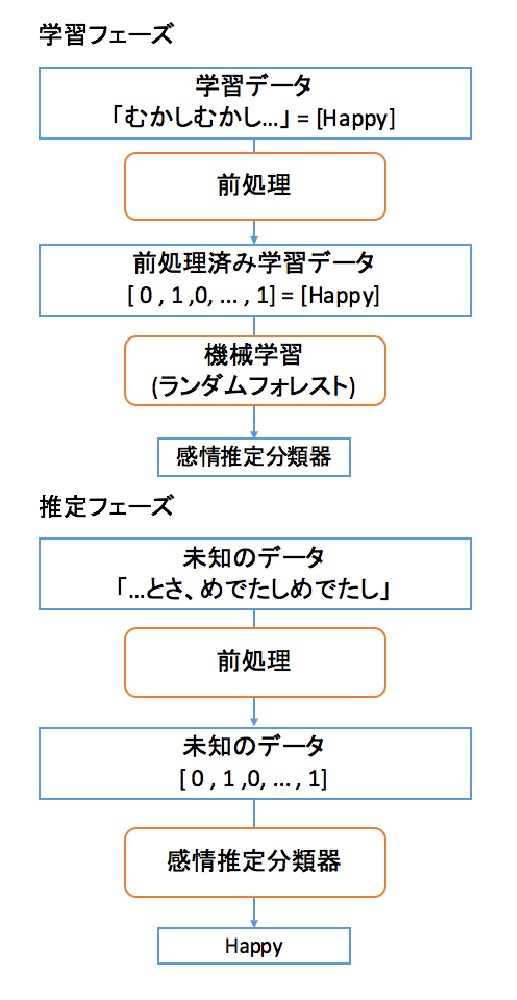
\includegraphics[clip,width=13.0cm]{fig/method-2.eps}
    \caption{提案手法の概要}
    \label{fig:method}
  \end{center}
\end{figure}

提案手法の概要を図\ref{fig:method}に示す.
本手法では,物語中のすべての文に対し文中に含まれる単語の出現を手がかりに朗読に最も適切もしくは自然と感じる感情を推定する.
感情のクラスはNormal,Happy,Sad,Angryの4種類とした.
まず,学習データとして各文に,それぞれ適切と思われる感情を人手で割り当てたものを用意する.
これに対し前処理を行いランダムフォレストを用いて学習を行う.
そして未知の入力文が与えられた場合に,感情クラスの1つを自動的に推定する他クラス分類を行うのが本手法である.

\section{前処理}

\begin{figure}[ht]
  \begin{center}
    \includegraphics[clip,width=10.0cm]{fig/method.eps}
    \caption{前処理の手順}
    \label{fig:pre}
  \end{center}
\end{figure}

機械学習で
前処理の手法を順に追って説明する.
その概要を図\ref{fig:pre}に示す.


\subsection{文の分割}\label{subsec:divide}
本手法では文単位で感情の推定を行う.
それゆえ,物語の文章を文に分ける必要がある.
意味内容を解読しそれにしたがって分割した方が自然な読み上げが可能になる可能性はあるが,朗読システムの構築を考えると単純な分割が好ましいと判断した.
基本的に,句点で文章を分ける.
カギ括弧で囲まれた箇所はそれを一文とし,その前後の文もそれぞれ一文とする.
%TODO 図で文分割を説明

\subsection{形態素解析}
次に文ごとに形態素解析を行う.
形態素解析とは文法的な情報の注記の無い自然言語の文から,文法や辞書と呼ばれる単語の品詞等の情報にもとづき,言語で意味を持つ最小単位である形態素の列に分割し,それぞれの形態素の品詞等を判別する作業である.
本手法では次節以降で述べる分かち書きと機能語の削除に形態素解析で得られた情報を用いる.

\subsection{分かち書き}
次に分かち書きを行う.
分かち書きとは文を語ごとにわける作業である.
英文の場合は語と語の間に空白(スペース)が入っているが,日本語の場合は入っていないため単純には行えない.
そこで前節の形態素解析の結果を用いて分かち書きを行う.

\subsection{内容語の削除}
本手法は,学習と推定の際に文から内容語(名詞,動詞,形容詞,形容動詞)を取り除き,機能語のみで推定を行う.
なぜならば,未知の物語の感情を推定を目的としているため,学習データが特定の物語に依存していては推定精度が低くとなると考えられるからである.
例えば「鬼」がネガティブに描かれている物語を学習データとして,別の「鬼」がポジティブに描かている物語を推定した場合にネガティブな感情に推定されてしまう恐れがある.
一方,機能後は「しまう」や「ところが」など,朗読時の抑揚などに関係すると考えられる重要な助詞や接続詞を含む.
したがって,内容語を排除し排除し,機能語のみで推定を行う.
このとき,形態素解析を行った結果を用いて,内容語と機能語の判別を行い内容語はデータから削除する.

\subsection{単語列のベクトル化}
分かち書きされた文を機械学習で扱える形式に変換がある.
本手法では,文のベクトル表現の1つであるbag-of-wordsを用いる.
解析で用いるすべての単語文の次元をもつベクトルを用意し文中に単語があれば1とし,なければ0とする.
なお今回は頻度は考慮せず,出現の否かのみを考慮する.

\section{機械学習}
\subsection{ランダムフォレスト}
一般に,入力データに対して,予め定義された複数のクラスから一つを推定する手法として機械学習の教師あり学習が適応できる.
本手法では,その中の手法の1つであるランダムフォレストを用いて機械学習を行う.
波部ら\cite{habe}によると,ランダムフォレストは複数の決定木を用いて森を構成し識別などを行う機械学習アルゴリズムである.
個々の決定木は高い識別性能をもつわけではないが,それらを複数用いてそれぞれの結果を補うことによって高い予測性能を得ることが1つの特徴である.
これは機械学習の分野ではアンサンブル学習と呼ばれており,個々の決定木がアンサンブル学習における弱識別器に相当する.
%TODO エントロピーの説明(数式)


\subsection{グリッドサーチ}
本手法ではより精度を向上させる手法として学習を行う前にグリッドサーチを行う.
グリッドサーチとは学習の際に与えるパラメタそれぞれに対していくつかの値を与え,それらの組み合わせについて学習と交差検証を行いつつ全探索し,最も良いスコアのパラメタを探索する手法である.
本手法で探索するパラメタは表\ref{parameter}の通りである.

\begin{table}[ht]
 \centering
  \caption{グリッドサーチで探索したパラメタの意味}
  \vspace{0.3\baselineskip}
     \scalebox{1}{
  \begin{tabular}{|c|c|} \hline
    パラメタ名&意味\\ \hline \hline
    max\_depth&木の最大の深さ\\ \hline
    n\_estimators&決定木の数\\ \hline
    max\_features&特徴量の最大の数\\ \hline
    criterion&重要度計算の尺度\\ \hline
    min\_sample\_split&葉ノードの最少分割数\\ \hline
    min\_samples\_leaf&葉ノードの特徴量の最小数\\ \hline
  \end{tabular}}
  \label{parameter}
\end{table}


\section{本章のまとめ}
本章では本研究で提案する文に対する感情推定の手法について,文章からベクトルへの変換手法や内容語削除などについて述べた.
次章では,本手法の有効性を示すための実験について説明する.


%--------------------------------------------------
%     第4章 実装
%--------------------------------------------------
\chapter{データセット}
本章では実験に用いる教師データを収集するためのシステムや集計手法について説明する.
教師データの作成手順を図\ref{fig:enquete}に示す.
本研究には,文に対してどの感情表現で音声合成を行うべきかという,文と感情表現ラベルが対になった学習データが必要である.
このために,物語文を元に各感情を指定した音声データを生成し,Webのアンケートシステムを用いて複数の評価者に評価してもらい,学習データを作成する.

\begin{figure}[hb]
  \begin{center}
    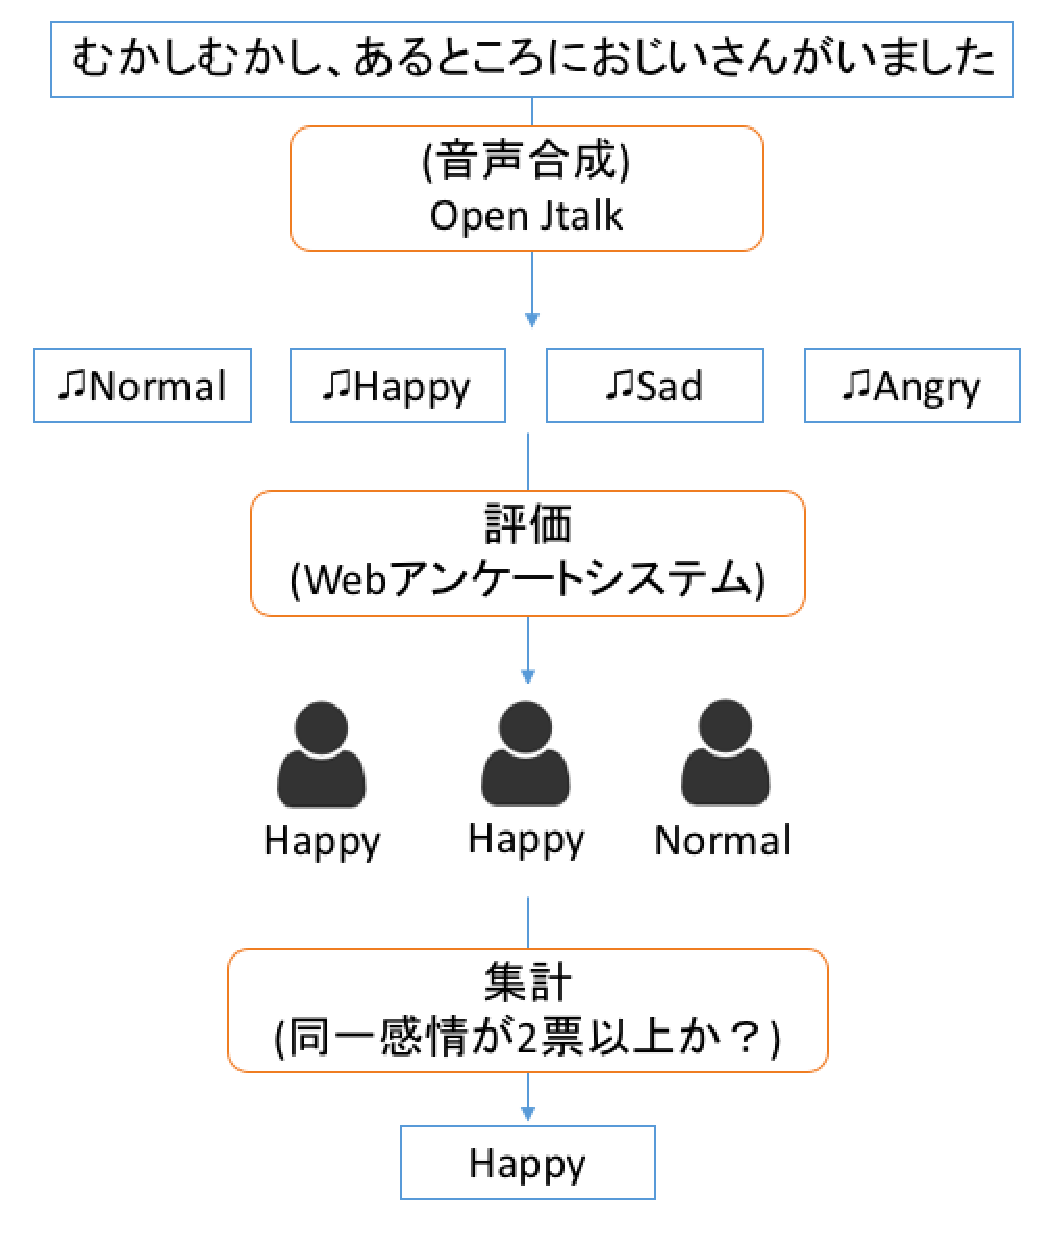
\includegraphics[clip,width=10.0cm]{fig/enquete.eps}
    \caption{学習データの作成手順}
    \label{fig:enquete}
  \end{center}
\end{figure}

\section{物語文章}
本実験では物語データとして,青空文庫\cite{aozora}にある5つの物語を用いる.
青空文庫とは,著作権が消滅した作品や著者が許諾した作品のテキストを公開しているインターネット上の電子図書館である
今回は文体を近づけるために同じ訳者の童話を中心に「白雪姫」,「赤ずきんちゃん」,「浦島太郎」,「ジャックと豆の木」,「ヘンゼルとグレーテル」を用いた.
%TODO 著者などを添えた表

\section{音声データの作成}
\subsection{前処理}

\begin{figure}[hb]
  \begin{center}
    \includegraphics[clip,width=14.0cm]{fig/aozora-convert.eps}
    \caption{青空文庫データの文分割とタグ削除処理}
    \label{fig:aozora-convert}
  \end{center}
\end{figure}


\ref{subsec:divide}で述べたように物語の文章を文に分ける.
朗読システム実現するためにはこの処理も自動化する必要がある.
また,青空文庫の書籍データにはルビや改行といったHTMLタグが挿入されているためこれを除く必要がある.
プログラミング言語Ruby\cite{ruby}を用いて,これらの処理を実装した.
これらの処理の例を\ref{fig:aozora-convert}に示す.

\subsection{音声合成ソフト}
本研究では音声合成にオープンソフトのOpen JTalk\cite{jtalk}を用いる.
Open Jtalkは日本語テキスト向けのHMM型の音声合成のオープンソースのソフトウェアである.
\ref{hmm-emotion}で述べた通りHMM型音声合成手法は少ない学習データで感情表現が可能になっている.
また,再現実験を考慮し広く利用が可能なオープンソースソフトウェアであるOpen Jtalkを用いた.

%TODO バクについて


音声波形データにはMMDAgent\cite{mei}にあるMeiのサンプルを用いた.
この音声波形データは1人の女性の848文の音声サンプルをもとに作成されている.
そのうち,503文は音声波形作成に広く用いられている用いられるATR音素バランス503文\cite{atr}であり,残りのうち215文は普通の発話スタイルで,残る75文は4つの感情(Angry, Bashful, Happy, Sad)の発話スタイルで収録されている.
それゆえ,MMDAgentにはNormal, Angry, Bashful, Happy, Sadの5つの音声波形データが用意されている.
本研究では布目ら\cite{fume}などの研究に従い,このうちのNormal, Angry, Happy, Sadの4つを利用した.


発音辞書にはNAIST Japanese Dictionary\cite{naist}を用いる.

各ソフトウェアの仕様は表\ref{voice-software}に示す.
\begin{table}[ht]
  \begin{center}
  \caption{音声合成のソフトウェア仕様}
  \label{}
  \begin{tabular}{|c|l|}
    \hline
    名称 & バージョン \\ \hline \hline
    Open JTalk & 1.10 \\ \hline
    NAIST Japanese Dictionary & 0.4.3  \\ \hline
    MMDAgent & 1.7 \\ \hline
  \end{tabular}
  \end{center}
\end{table}

\subsection{音声データファイル}
本研究では,前章のOpen JTalkとMeiの音声波形データ等を用いて,一つの文に対して4つの異なる感情表現の音声ファイルを生成する.
この音声ファイルはWAVフォーマット形式で出力される.
WAVフォーマット形式は,非圧縮形式でありリニアPCMのサンプリングデータ用のフォーマットとして扱われる.
Open JTalkの出力ではサンプルレートが48,000Hz,16bps,モノラルのWAVファイルが得られる.
%TODO ↑表にする??

\section{アンケートシステム}

本研究では効率よく学習データを採取するためにWeb上で文に対して感情のラベル付けが行えるシステムを構築した.

\subsection{システムの概要}
\begin{figure}[h]
  \begin{center}
    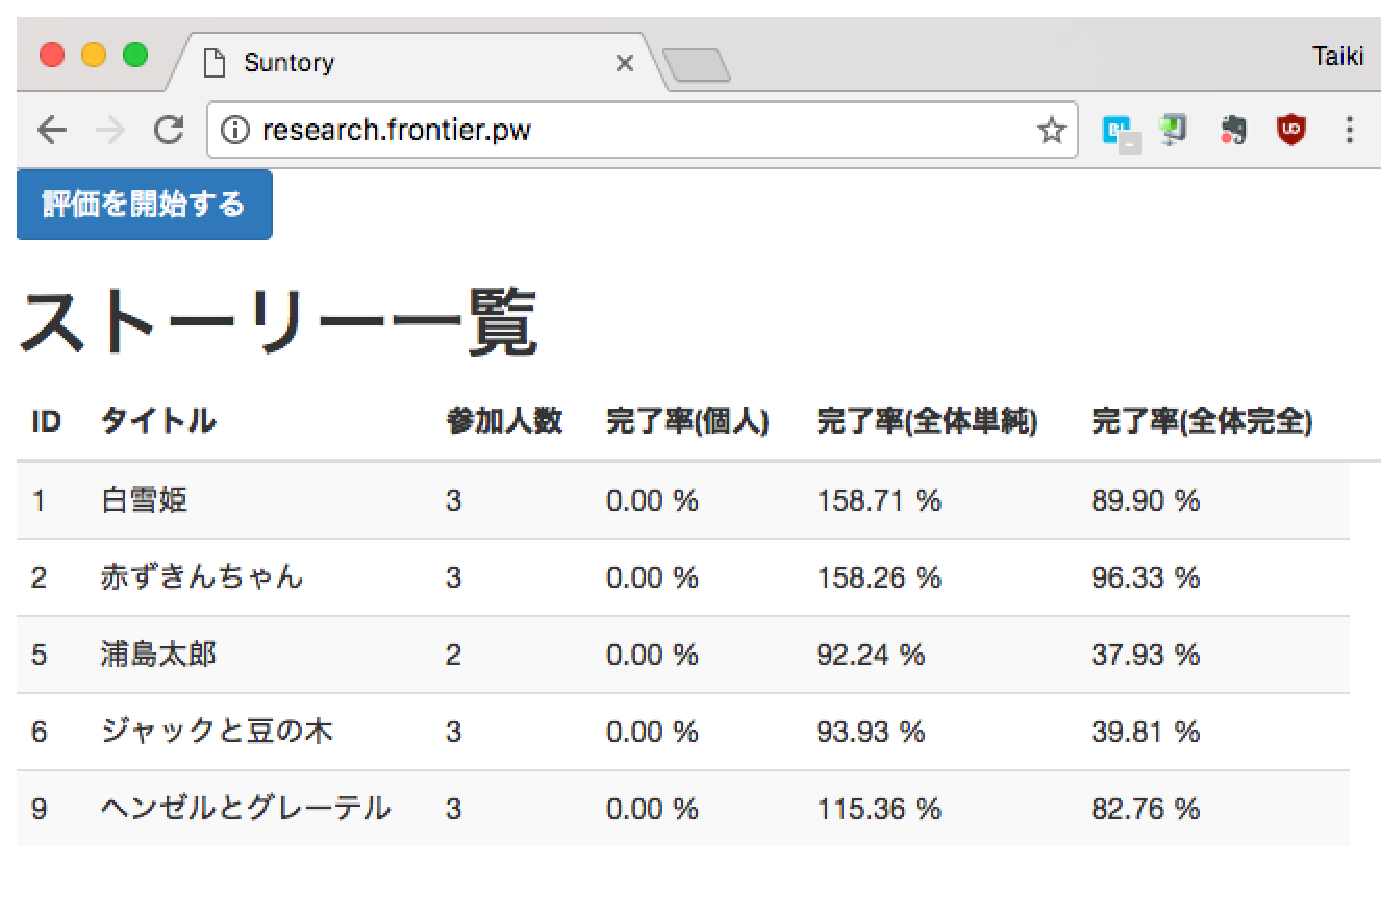
\includegraphics[clip,width=13.0cm]{fig/web-index.eps}
    \caption{WEBアンケートシステム選択画面}
    \label{fig:index-web}
  \end{center}
\end{figure}

\begin{figure}[h]
  \begin{center}
    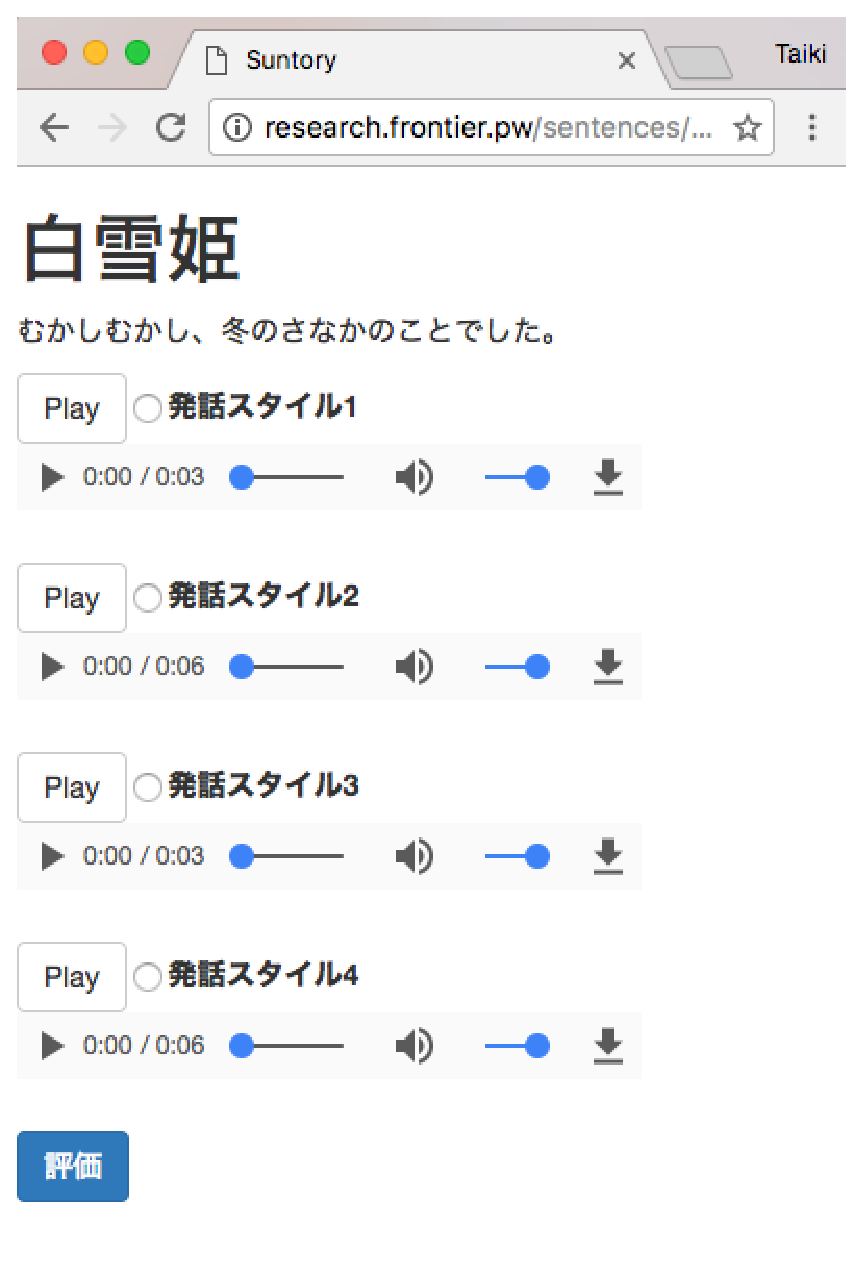
\includegraphics[clip,width=10.0cm]{fig/web.eps}
    \caption{WEBアンケートシステム評価画面}
    \label{fig:web}
  \end{center}
\end{figure}
サインアップもしくはログインを行い評価者は図\ref{fig:index-web}のインデックスページの評価ボタンがから図\ref{fig:web}に示す評価ページに遷移する.
評価ページにおいて後述する評価アルゴリズムに基づいて自動選択された文について評価者は4つの音声それぞれを聞き,内容にもっとも適切(自然)であると思われる感情を1つだけ選択してもらう.
評価ボタンをクリックすると評価はデータベースに保存され,自動選択された別の文の評価ページへと遷移する.

\subsection{システムの利用技術}
WebアプリケーションフレームであるRuby on Rails\cite{rails}を採用し,データベースにはSQlite3\cite{sqlite}を用いた構築した.

評価ページの音声再生部分にはHTML5に定められているWeb Audio APIとaudioタグによる2つの実装を行った.
これは,評価者のブラウザ環境によってはどちらかが使えない場合があるからである.
なお,Playボタンを押すとWeb Audio APIが呼び出されるがこの部分の実装にはJavaScriptを用いた.
これにより,Open JTalkで生成されたWAVファイルが評価自身の端末で再生可能となった.

また,得られた学習データはCSV形式で出力する機能も備えており実用的である.

その他,本システム用いたサーバー機のスペックはソフトウェアの仕様\ref{software}に,表\ref{server}に示す

\begin{table}[ht]
  \begin{center}
  \caption{アンケートシステムのソフトウェア仕様}
  \label{software}
  \begin{tabular}{|c|l|}
    \hline
    名称 & バージョン \\ \hline \hline
    Ruby & 2.3.3p222 \\ \hline
    Ruby on Rails & 4.2.7.1 \\ \hline
    SQLite3 & 3.7.17 \\ \hline
  \end{tabular}
  \end{center}
\end{table}

\begin{table}[ht]
  \begin{center}
  \caption{アンケートシステムのサーバースペック}
  \label{server}
  \begin{tabular}{|c|l|}
    \hline
     名称 & スペック \\ \hline \hline
    マシン &  マウスコンピューター MASTERPIECE i1550PA7-CL-W7\\ \hline
    OS &  CentOS Linux release 7.3.1611 (Core)\\ \hline
    CPU & Intel Core i7-3970X 3.50GHz × 2\\ \hline
    メモリサイズ & 64.0GB \\ \hline
  \end{tabular}
  \end{center}
\end{table}



\subsection{評価アルゴリズム}
被験者には文ごとに各感情のパラメタで合成した音声をそれぞれ聞いてもらい,内容にもっとも適切(自然)であると思われる感情を1つだけ選択してもらう.
しかし,感情は主観的な尺度であるため1人だけの評価では信頼性が低い.
そこで,一文に対して同じ感情の評価が2票集まった時点で評価を確定することとした.
異なる評価が集まった場合はもう1票だけ評価を続け,既存の評価と同じ感情であればその評価で確定することにした.
3票ともに異なる評価が集まった場合には,その文は学習データとしては利用しないこととした.
なお,セリフ文を優先的に評価するように設定した.


\subsection{学習データの収集}
大学生に自身が所有するPCやスマートフォンで,アンケートシステムにアクセスさせ,評価を行わせた.
なお,評価の期限や数は評価者の任意とした.
その他詳細は表\ref{enviroment}に示す.

\begin{table}[ht]
  \begin{center}
  \caption{学習データの収集}
  \label{enviroment}
  \begin{tabular}{|c|l|}
    \hline
    被験者 & 東京理科大学の学部生及び大学院生 \\ \hline
    人数 & 学部生15名,大学院生2名 \\ \hline
    取得期間 & 2017年1月9日〜25日 \\ \hline
    評価取得数 & 2641 \\ \hline
  \end{tabular}
  \end{center}
\end{table}



\section{学習データの概要}
学習データの概要を表\ref{sentence-count}と表\ref{emotion-count}に示す.

全体で評価が確定したものは全体で69.8\%であった.
セリフは全体の33.21\%であり,セリフの評価完了率は81.04\%であった.
表\ref{emotion-count}の通り,Normal以外の感情はセリフに多く含まれており,セリフの方が感情豊かであり,それ以後の文はNormalであることが多いことがわかる.

\begin{table}[ht]
 \centering
  \caption{学習データ(物語別)}
  \vspace{0.3\baselineskip}
  \scalebox{0.8}{
  \begin{tabular}{|c|c|c|} \hline
    タイトル & 文数(セリフ) & 評価確定数(セリフ) \\ \hline \hline
    白雪姫 & 287 (90) & 258 (86)   \\ \hline
    赤ずきんちゃん & 109 (54) & 108 (54)   \\ \hline
    浦島太郎 & 206 (48) & 78 (26)   \\ \hline
    ジャックと豆の木 & 206 (49) & 78 (26)   \\ \hline
    ヘンゼルとグレーテル & 319 (114) & 260 (90)   \\ \hline\hline
    合計 & 1096 (364) & 765 (283) \\ \hline
  \end{tabular}
  }
  \label{sentence-count}
\end{table}

\begin{table}[ht]
 \centering
  \caption{学習データ(感情別)}
  \vspace{0.3\baselineskip}
  \scalebox{0.90}{
  \begin{tabular}{|c|c|c|} \hline
    感情 & 全文 & セリフのみ  \\ \hline \hline
    Normal & 459  & 63  \\ \hline
    Happy & 134 & 110 \\ \hline
    Sad & 99  & 60  \\ \hline
    Angry & 73  & 50  \\ \hline \hline
    合計 & 765 &  283 \\ \hline
  \end{tabular}
  }
  \label{emotion-count}
\end{table}

\section{本章のまとめ}
本章では,本研究に用いるデータセットの説明や収集方法,アンケートシステムの詳細について説明した.





%--------------------------------------------------
%     第5章 評価と考察
%--------------------------------------------------
\chapter{評価}

本章では提案手法を具体的に実装したシステムを用いて,主要コンテンツの抽出性能を評価するために行なった実験の概要と結果について述べる.

\section{評価目的}



%--------------------------------------------------
%     第6章 結論
--------------------------------------------------
\chapter{結論}

本研究では未知の文に対しその文を読み上げるときの感情として最適なものを推測することを目的とした.
このための手法として物語に依存しがちな内容語を除いて機能語のみを用いてランダムフォレストで学習・推定する手法を提案した.


実験はネット上の5つの物語を使用して音声データを作成しWebのアンケートシステムを用いてNormal,Happy,Sad,Angryの4つのに分類し学習データを作成した.
また,比較実験として機能語のみで学習・推定するか否かやランダムフォレストの他にSVMでの実験やセリフ文のみに絞った場合を行った.


結果とした全体的に高い精度を得ることはできなかった.
しかし,本研究にはSVMよりランダムフォレストが有用であることや内容語を取り去って機能語のみで学習・分類を行っても,精度に大差はないことがわかった.
したがって,ランダムフォレストを用いて,物語を増やし学習データを増やして学習を行い未知の物語に対して推定する検証を行うことで本手法の有用性が証明される可能性がある.




%--------------------------------
%     参考文献
%--------------------------------
\markright{参考文献}
\begin{thebibliography}{99}

%TODO 順番確認
% http://ci.nii.ac.jp/naid/110009971766
\bibitem{wsj} Jennifer Maloney,"The Fastest-Growing Format in Publishing: Audiobooks",http://www.wsj.com/articles/the-fastest-growing-format-in-publishing-audiobooks-1469139910,Wall Steet Journal
\bibitem{cnet} 佐藤和也,"高い継続率は「耳がさみしくなるから」--オトバンクに聞くオーディオブック市場と利用動向",https://japan.cnet.com/article/35076656/
\bibitem{ueda} 上田渉,"「耳で聴く読書文化」を築く",http://www.ajec.or.jp/interview\_width\_ueda1/,一般社団法人日本編集制作協会
\bibitem{sugifuji} 杉藤美代子; 大山玄. 朗読におけるポーズと呼吸―息継ぎのあるポーズと息継ぎのないポーズ―. 音声言語. 1990.
\bibitem{yoshimura} YOSHIMURA, Takayoshi. Simultaneous modeling of phonetic and prosodic parameters, and characteristic conversion for HMM-based text-to-speech systems. 2002. PhD Thesis. Nagoya Institute of Technology.
\bibitem{iida} 飯田朱美, and 安村通晃. "感情表現が可能な合成音声の作成と評価." 情報処理学会論文誌 40.2 (1999): 479-486.
\bibitem{tsuduki} 都築亮介, et al. HMM 音声合成における感情表現のモデル化 (合成, 韻律, 生成, 一般). 電子情報通信学会技術研究報告. SP, 音声, 2003, 103.264: 25-30.
\bibitem{habe} 波部斉,”ランダムフォレスト”,情報処理学会研究報告 2012

\bibitem{yoshida} 吉田有里,奥平康弘,田村直良,”音声合成による朗読システムに関する研究”,情報科学技術フォーラム講演論文集,2009:p337-380
\bibitem{otani} 大谷大和, et al. "HMM に基づく感情音声合成のための共有感情付与モデル (オーガナイズドセッション 「文脈や状況に合った発声を実現する音声合成技術及び周辺技術」, 合成, 韻律, 生成, 音声一般)." 電子情報通信学会技術研究報告. SP, 音声 114.303 (2014): 13-18.
\bibitem{fume} 布目光生,鈴木優,森田眞弘,”自然で聞きやすい電子書籍読上げのための文書構造解析技術,東芝レビュー,2011:p32-35
\bibitem{aozora} 青空文庫,http://www.aozora.gr.jp/
%TODO 他の文も
%\bibitem{shirayuki} グリム,菊池寛訳,”白雪姫”,http://www.aozora.gr.jp/cards/001091/files/42308\_17916.html

%ちゃんとした形式に直す
\bibitem{jtalk} 大浦 圭一郎,酒向 慎司, 徳田 恵一,”日本語テキスト音声合成システム Open JTalk”,日本音響学会春季講論集,2010:p343-344
\bibitem{mecab} "MeCab: Yet Another Part-of-Speech and Morphological Analyze",http://taku910.github.io/mecab/
\bibitem{naist} "NAIST Japanese Dictionary",http://naist-jdic.osdn.jp/
\bibitem{mei} "MMDAgent",http://www.mmdagent.jp/


\end{thebibliography}


%--------------------------------
%     アペンディクス
%--------------------------------
\appendix
\chapter{WebページのURLリスト}
\vspace{-15mm}


\end{document}
